\subsection{Two additional count datasets and a limit of the certificate}
\label{sec:multidata}
We add Seoul Bike Sharing Demand~\cite{seoul} and Metro Interstate
Traffic Volume~\cite{metro}. The official files, their SHA-256 values,
and CC BY 4.0 attribution are retained. A stable chronological sort
followed by the first 80\% of rows gives 7008 Seoul observations with
15 model coordinates and 38563 Metro observations with 12 coordinates.
Repeated source timestamps retain their original weights.
Fixed feature choices include weather, cyclic time features, holiday,
and Seoul's functioning indicator; other textual categories are omitted.
Each non-intercept feature becomes
$\tanh((v-\bar v_{\rm train})/s_{\rm train})$ using training statistics
only. This bounded-feature protocol differs from the earlier Bike
Sharing standardization. Predictive accuracy is not evaluated.

The normalized Poisson deviance and ridge coefficient $\mu=0.01$ are
as before; the intercept is also constrained and regularized. Since
$\norm{a_i}_\infty=1$ and the normalized response $t_i$ has mean one,
valid radius-$R$ bounds are
\[
 H_1=\max_i\norm{a_i}^2,\quad H_0=\mu+H_1(1+R),\quad
 L_Q=\mu+e^R\lambda_{\max}(A^\top A/m).
\]
The Hessian norm is at most
$\mu+H_1\operatorname{mean}(e^{a_i^\top x})$; comparing $f_Q^*$ with
$f(0)$ yields $\operatorname{mean}(e^{a_i^\top x})\le\delta+1+R$.
Thus the condition holds relative to the constrained minimum. These
are upper bounds, not minimal curvature parameters, and positive
$H_1$ is not claimed necessary on a compact domain.

Offline damped Newton solves estimate $R_*:=\norm{x^*_{\rm unc}}_1$.
The values are approximately 4.575821 (Seoul) and 1.431745 (Metro). We compare
$R/R_*=1/2$ and 2, with independently recomputed active and interior
reference intervals of width below $4.3\cdot10^{-8}$. All 30 Seoul or
24 Metro signed coordinate vertices are used once per radius. Six
existing variants give 648 trajectories: the four BT variants and
FW/AFW known-$H$ short steps. The cap is 1000 updates, the tolerance
$10^{-5}$. References, activity and $R_*$ are offline information, not
solver inputs. Starts and radii within each dataset share data.

Both AFW-BT variants finish all 30 active Seoul and all 24 active Metro
starts. Their function-call medians are 424 versus 399 and 99 versus
80.5 for $M=1$ versus $M=U_0/D^2$, respectively. The interior controls
are unfavorable: neither AFW-BT variant finishes any Seoul start,
and only 6/24 and 7/24 finish on Metro. AFW-Q finishes all active Metro
starts with median 423 function/gradient calls, but no start in the
other three cases. These results limit any practical-success claim
based on the earlier Bike Sharing controls. All full trajectories
pass descent, feasibility, trial-count, active-removal, and local-gap
checks before sampling.

The independent reference interval distinguishes primal error from
the online certificate. At the interior Metro radius, every BT run
has post-run upper error
$e_{\rm ref}=\max\{0,f(x)-f^*_{\rm ref,lower}\}\le10^{-5}$.
Yet FW has no online $U$ successes and AFW has only 6 and 7. On
interior Seoul, 12/30 and 18/30 AFW runs have $e_{\rm ref}\le10^{-5}$,
although neither variant stops. Noncompletion can therefore reflect
both remaining primal error and a conservative observable certificate.
References do not replace actual stopping outcomes. Tighter dual
certificates merit investigation with their extra linear oracles
properly counted. Active-set work is additional, and no wall-clock
ranking follows from these counts.

\begin{table}[htbp]
\centering\small
\caption{Additional count datasets, every signed coordinate vertex. Entries: successes; median final function calls including failures capped at 1000 updates. Seoul has 30 starts per radius, Metro 24. $F/A$: FW/AFW; subscripts $1,U$: initial $M=1,U_0/D^2$; $Q$: known-$H$ short step.}
\label{tab:multidata}
\begin{tabular}{lrrrrrr}
\hline
$R/R_*$ & $F_1$ & $F_U$ & $A_1$ & $A_U$ & $F_Q$ & $A_Q$ \\
\hline
\multicolumn{7}{l}{\textbf{seoul}} \\
0.5 & 1; 2001 & 1; 2003 & 30; 424 & 30; 399 & 0; 1001 & 0; 1001 \\
2 & 0; 2001 & 0; 1996 & 0; 2001 & 0; 1995.5 & 0; 1001 & 0; 1001 \\
\hline
\multicolumn{7}{l}{\textbf{metro}} \\
0.5 & 3; 2001 & 3; 2003 & 24; 99 & 24; 80.5 & 1; 1001 & 24; 423 \\
2 & 0; 2000 & 0; 2002 & 6; 2000 & 7; 2001 & 0; 1001 & 0; 1001 \\
\hline
\end{tabular}
\end{table}

\begin{figure}[htbp]
\centering
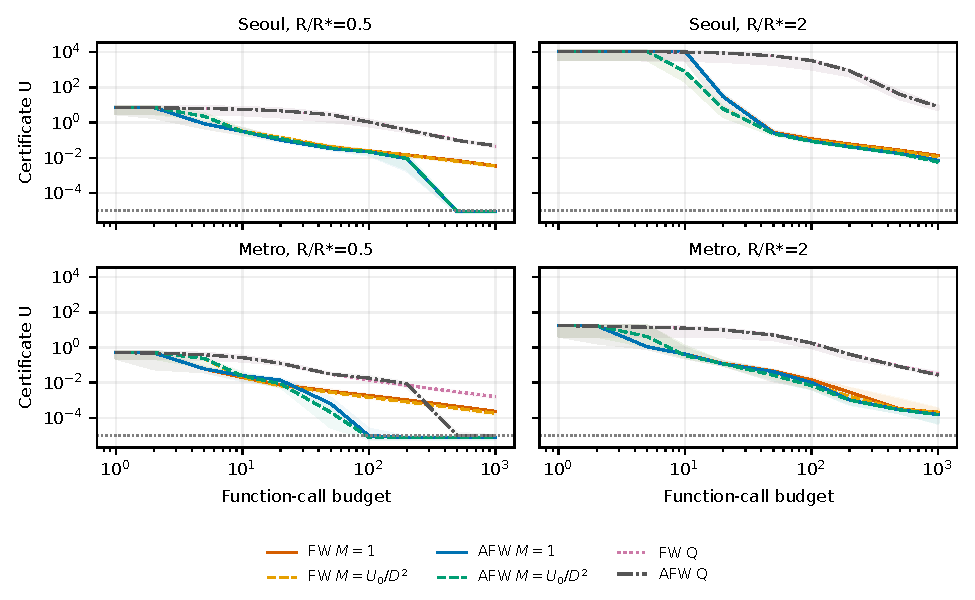
\includegraphics[width=\textwidth]{figures/additional_counts.pdf}
\caption{Additional real count datasets. Median certificate and
interquartile band over every signed coordinate vertex, at separate
function-call budgets. Completed runs are carried forward; nonterminal
runs reach the displayed budgets. BT has no curvature inputs; Q receives
analytic $H_0,H_1$. Radii and starts within a dataset share training data.}
\label{fig:multidata}
\end{figure}
